\documentclass[border=6pt]{standalone}
\usepackage{newtxtext,newtxmath}
\usepackage{tikz}
\usetikzlibrary{arrows.meta}
\tikzset{
  axis/.style={-{Stealth[length=5pt,width=4pt]}, line width=0.45pt},
  curve/.style={line width=0.8pt},
  guide/.style={dashed, line width=0.4pt, dash pattern=on 2pt off 1.5pt},
  dot/.style={circle, fill, inner sep=0pt, minimum size=3.2pt},
}
\begin{document}
% ---------- 1. 이차함수 y = x^2 - 2x - 3 ----------
\begin{tikzpicture}[scale=0.62]
  \draw[axis] (-2.6,0) -- (4.6,0) node[right] {$x$};
  \draw[axis] (0,-5) -- (0,5.6) node[above] {$y$};
  \node[below left, inner sep=1.5pt] at (0,0) {$O$};
  \draw[curve, domain=-1.75:3.75, samples=80, smooth] plot (\x, {\x*\x-2*\x-3});
  \draw[guide] (1,0) -- (1,-4) -- (0,-4);
  \node[dot] at (-1,0) {}; \node[dot] at (3,0) {}; \node[dot] at (1,-4) {};
  \node[below left, inner sep=2pt] at (-1,0) {$-1$};
  \node[below right, inner sep=2pt] at (3,0) {$3$};
  \node[above, inner sep=2pt] at (1,0) {$1$};
  \node[left, inner sep=2pt] at (0,-4) {$-4$};
  \node[right] at (3.75,4.6) {$y=f(x)$};
\end{tikzpicture}
\hspace{1.2cm}
% ---------- 2. 삼차함수 y = x(x-2)(x-3), 0~2 넓이 ----------
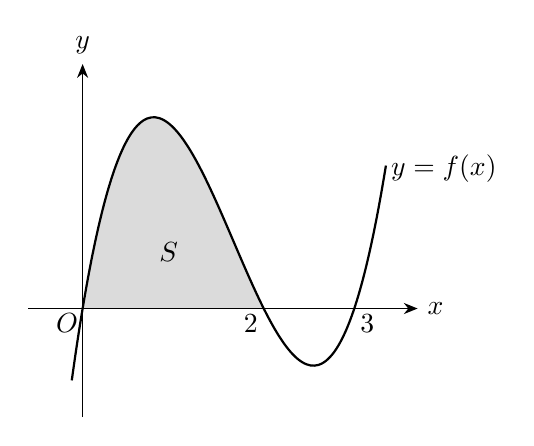
\begin{tikzpicture}[scale=1.15]
  \fill[gray!28, domain=0:2, samples=60, smooth] plot (\x, {\x*(\x-2)*(\x-3)}) -- (2,0) -- (0,0) -- cycle;
  \draw[axis] (-0.6,0) -- (3.7,0) node[right] {$x$};
  \draw[axis] (0,-1.2) -- (0,2.7) node[above] {$y$};
  \node[below left, inner sep=1.5pt] at (0,0) {$O$};
  \draw[curve, domain=-0.12:3.35, samples=80, smooth] plot (\x, {\x*(\x-2)*(\x-3)});
  \node[below left, inner sep=2pt] at (2,0) {$2$};
  \node[below right, inner sep=2pt] at (3,0) {$3$};
  \node at (0.95,0.62) {$S$};
  \node[right] at (3.3,1.55) {$y=f(x)$};
\end{tikzpicture}
\end{document}
